\section{Theoretical Results for Scalar Conservation Laws}
\label{sec:method}
In this section, we are concerned with solving problems of the following form: Find $u \in L^{\infty}((0,\tend); \mathbb{T})$ such that
\begin{equation}
\begin{cases}
\partial_t u + \partial_x f(u) = 0&\\
u(x,0) = u_0(x),&
\end{cases}
\label{eq:ivp}
\end{equation}
where $f$ is a Lipschitz flux, $u_0(x) \in L^{\infty}(\mathbb{T})\cap BV(\mathbb{T})$, and $\mathbb{T}$ is the unit torus.  Consider a finite partitioning of the torus, $\Omega^h = \cup_{j=0}^{n_{el}} (x_j,x_{j+1})$ as defined by the strictly increasing sequence ${x_j} \subset (0,1)$. Let $U_j$ denote the average value on the interval $(x_j, x_{j+1})$, and let $\Delta$ denote the forward difference operator, i.e.
\begin{equation*}
\Delta U_k = U_{k+1} - U_k.
\end{equation*}
We specify an approximation to the conservation law as a set of pairs,
\begin{equation*}
\mathcal{E} = \left\{ (t_j^n, U_j^n)\,:\, 0 \le j \le n_{el},\,n\in\mathbb{R}_+ \right\},
\end{equation*}
where $U_j^n$ is the average value over the cell $(x_j,x_{j+1})$ at time $t_j^n$. We refer to this collection of space-time points as the {\em event trace}. We define the timestamps $\mathcal{T}_j$ on cell $j$, as
\begin{equation*}
\mathcal{T}_j = \left\{ t_j^* \, : \, \exists\, U_j^* \, \text{s.t.}\, (t_j^*,U_j^*) \in \mathcal{E} \right\}.
\end{equation*}
We define for cell $j$, the nearest previous timestep for time $t$ as
\begin{equation*}
\lfloor t \rfloor_j = \max \{ \tau \in \mathcal{T}_j \, : \, \tau \le t \}.
\end{equation*}
We similarly define the next timestep at time $t$ as
\begin{equation*}
\lceil t \rceil_j = \min \{ \tau \in \mathcal{T}_j\, : \, \tau > t \}.
\end{equation*}
To achieve the desired theoretical results, we impose two constraints on the event traces. Firstly, we assume that there are only a finite number of events. Secondly, we need to restrict when timestamps are able to step relative to one another. 

We call the set of timestamps $\cup_j \mathcal{T}_j$ \emph{locally ordered} if for each cell $j$ there exists a sequence of pairwise synchronization times $\{s^{\mu}_{j,j+1}\}_{\mu=0}^{n_s} \subset \mathcal{T}_j \cap \mathcal{T}_{j+1}$ such that for all consecutive synchronization times $s^{\mu}_{j,j+1}$ and $s^{\mu+1}_{j,j+1}$, either
\begin{equation*}
\mathcal{T}_j \cap (s^{\mu}_{j,j+1}, s^{\mu+1}_{j,j+1}) = \emptyset \quad\text{or}\quad \mathcal{T}_{j+1} \cap (s^{\mu}_{j,j+1}, s^{\mu+1}_{j,j+1}) = \emptyset.
\end{equation*}
That is to say that one cell must step strictly faster than its neighbor between  synchronization times. To illustrate this definition, we've drawn a sketch of potential local timestepping solutions in Figure \ref{fig:sol-cartoon}.
\begin{figure}
\centering
\subfloat[Straddling]{
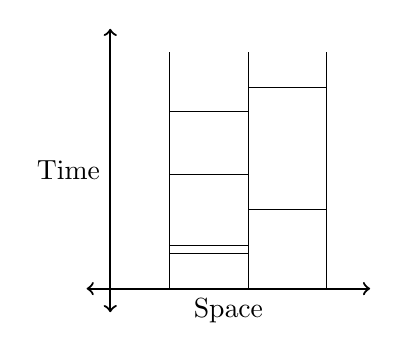
\begin{tikzpicture}
    \draw[<->,thick] (-0.3,0)--(3.3,0) node[midway,below] {Space};
    \draw[<->,thick] (0,-0.3)--(0,3.3) node[midway,left] {Time};
    \draw[-] (0.75,0)--(0.75,3);
    \draw[-] (1.75,0)--(1.75,3);
    \draw[-] (2.75,0)--(2.75,3);
    \draw[-] (0.75, 0.45)--(1.75, 0.45);
    \draw[-] (0.75, 0.55)--(1.75, 0.55);
    \draw[-] (0.75, 1.45)--(1.75, 1.45);
    \draw[-] (0.75, 2.25)--(1.75, 2.25);
    \draw[-] (1.75, 1)--(2.75, 1);
    \draw[-] (1.75, 2.55)--(2.75, 2.55);
\end{tikzpicture}
}\hspace{1in}
\subfloat[Locally Ordered]{
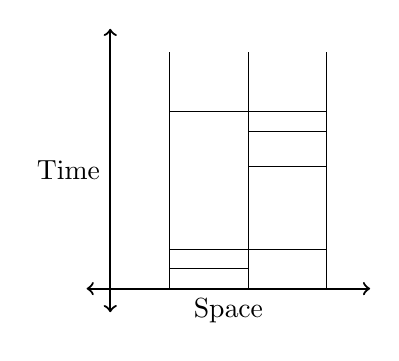
\begin{tikzpicture}
    \draw[<->,thick] (-0.3,0)--(3.3,0) node[midway,below] {Space};
    \draw[<->,thick] (0,-0.3)--(0,3.3) node[midway,left] {Time};
    \draw[-] (0.75,0)--(0.75,3);
    \draw[-] (1.75,0)--(1.75,3);
    \draw[-] (2.75,0)--(2.75,3);
    \draw[-] (0.75, 0.25)--(1.75, 0.25);
    \draw[-] (0.75, 0.5)--(1.75, 0.5);
    \draw[-] (0.75, 2.25)--(1.75, 2.25);
    \draw[-] (1.75, 0.5)--(2.75, 0.5);
    \draw[-] (1.75, 1.55)--(2.75, 1.55);
    \draw[-] (1.75, 2)--(2.75, 2);
    \draw[-] (1.75, 2.25)--(2.75, 2.25);
\end{tikzpicture}
}
\caption{Comparison of two event traces.}
\label{fig:sol-cartoon}
\end{figure}
Additionally, we define the value of an approximation at any point in time and space as the most recent average value of the cell containing the given point, i.e. 
\begin{equation*}
U(t,x) = \begin{cases}
U_j^n & \text{if } x \in (x_j, x_{j+1}) \quad \text{and} \quad t = t_{j^n},\\
U(\tprev_j, x) & \text{where } x \in (x_j, x_{j+1}).
\end{cases}
\end{equation*}
We also introduce $U_j(t)$ as the value of the solution $U(x,t)$ inside cell $j$ at time $t$. To approximate the flux exchange at the boundary, we define a numerical flux $\hat{F}(\cdot, \cdot)$. Additionally, we require that the numerical flux be:
\begin{enumerate}
\item {\em Consistent}, i.e. $\hat{F}(u^*,u^*) = f(u^*)$,
\item {\em Monotone}, i.e. $\hat{F}$ is increasing in the first argument, and decreasing in the second argument,
\item {\em Lipschitz continuous} in both arguments.
\end{enumerate}
We now define the Euler approximation to the scalar conservation law as follows.
\begin{definition}[Forward Euler Approximation]
An event trace $\mathcal{E}$ is an Euler approximation to the scalar conservation law if
\begin{equation}
U_j^{n+1} = U_{j}^n + \frac{1}{\Delta x_j}\int_{t_j^n}^{t_j^{n+1}} \big[ \hat{F}(U_{j-1}(\tau), U_j^n) - \hat{F}(U_j^n,U_{j+1}(\tau)) \big] \,\mathrm{d}\tau,
\label{eq:update}
\end{equation}
for all cells $j$, and between all updates $t_j^n$ and $t_j^{n+1}$, where $\hat{F}$ is a numerical flux.
\end{definition}

The remainder of this section assumes the existence of forward Euler approximations. Under this assumption, we present proofs that under CFL-like constraints, a maximum principle and total variation stability can be obtained. We note that the proofs follow closely the proof presented in~\cite{Osher1983,Kirby2003}. In the next section, we will present an algorithm which satisfies the assumptions of the theorems presented in this section.

Following the spirit of the analysis proposed in~\cite{Harten1983}, define
\begin{equation*}
C_j = - \left( \frac{ \hat{F}(U_j,U_{j+1}) - \hat{F}(U_{j-1},U_{j+1})}{\Delta x_j( U_j - U_{j-1})}\right) \text{ and } D_j = \frac{  \hat{F}(U_{j-1},U_{j+1}) - \hat{F}(U_{j-1},U_{j})}{\Delta x_j (U_{j+1} - U_{j})}.
\end{equation*}
We remark that due to the Lipschitz continuity of the numerical flux both $C_j$ and $D_j$ are bounded, and due to the monotonicity of the numerical flux $C_j \le 0 \le D_j$ for all $U_{j-1},U_j,U_{j+1}\in \mathbb{R}$. We reformulate the update rule \eqref{eq:update} as
\begin{equation}
U_j^{n+1} = U_j^n + \int_{t_j^n}^{t^{n+1}_j} \big[ C_j(\tau) \Delta U_{j-1}(\tau) - D_j(\tau) \Delta U_j(\tau) \big] \,\mathrm{d} \tau.
\label{eq:update2}
\end{equation}
Note that this representation is slightly different than the analyses presented in~\cite{Harten1983,Osher1983,Kirby2003}. We do not multiply our $C_j$ and $D_j$ coefficients by $\Delta t$.

\begin{theorem}[Maximum Principle]
Consider an event trace $\mathcal{E}$ satisfying the forward Euler approximation~\eqref{eq:update}. If given any two events $(t_j^n,\,U_j^n)$ and $(t_j^{n+1},\,U_j^{n+1})$,
\begin{equation}
1 + \int_{t_j^n}^{t_j^{n+1}} \big[ C_j(\tau) - D_j(\tau) \big] \,\mathrm{d}\tau \ge 0,
\label{eq:cfl-max}
\end{equation}
then
\begin{equation*}
|U^n_j| \le \sup_j |U^0_j|.
\end{equation*}
\label{thm:max}
\end{theorem}
\begin{proof}
Using the update criterion~\eqref{eq:update2},
\begin{equation*}
U^{n+1}_j = U_j^n + \int_{t_j^n}^{t_j^{n+1}} \big[ C_j(\tau) \Delta U_{j-1}(\tau) -D_j(\tau) \Delta U_j(\tau) \big] \, \mathrm{d}\tau
\end{equation*}
Using the CFL condition~\eqref{eq:cfl-max}, and $C_j(\tau) \le 0 \le D_j(\tau)$ for all $\tau$,
\begin{align*}
\left| U^{n+1}_j \right| & \le
\left| U_j^n + \int_{t^n_j}^{t^{n+1}_j} \big[ C_j(\tau) U_j^n - D_j(\tau)  U_j^n \big] \mathrm{d} \tau \right| \\
& \quad + \left| \int_{t^n_j}^{t^{n+1}_j} C_j(\tau) U_{j-1}(\tau) \mathrm{d} \tau \right| + \left| \int_{t^n_j}^{t^{n+1}_j} D_j(\tau) U_{j+1}(\tau) \mathrm{d} \tau \right|,\\
& \le \left( 1+ \int_{t^n_j}^{t^{n+1}_j} C_j(\tau)  + D_j(\tau) \, \mathrm{d} \tau \right) |U_j^n|\\
& \quad - \int_{t^n_j}^{t^{n+1}_j} C_j(\tau) |U_{j-1}(\tau)| \,\mathrm{d}\tau + \int_{t^n_j}^{t^{n+1}_j} D_j(\tau) |U_{j+1}(\tau)| \,\mathrm{d}\tau.
\end{align*}
Let $U^* = \sup_{\tau \in [t_j^n,t_j^{n+1})} \{ |U_j^n|, |U_{j-1}(\tau)|, |U_{j+1}(\tau)| \}$, then \
\begin{align*}
|U^{n+1}_j| & \le \left( 1 + \int_{t_j^n}^{t_j^{n+1}} \big[ C_j(\tau) - D_j(\tau) \big]\mathrm{d} \tau \right) U^* \\
& - \left(  \int_{t_j^n}^{t_j^{n+1}} C_j(\tau) \mathrm{d} \tau \right) U^* + \left(  \int_{t_j^n}^{t_j^{n+1}} D_j(\tau) \mathrm{d} \tau \right) U^*\\
& \le U^*.
\end{align*}

Lastly, we define the minimum time between events as
\begin{equation*}
\varepsilon = \inf_{j,k,n} \left\{ t_j^{n} - t \, : \, t \in \mathcal{T}_k \land t < t_j^n \right\}.
\end{equation*}
Since we've assumed a finite number of events, $\varepsilon>0$. Letting $\mathcal{U}(t)$ be defined as the largest value up till time $t$, i.e.
\begin{equation*}
\mathcal{U}(t) = \max_{j,\,\tau \le t} |U_j(\tau)|.
\end{equation*}
By the definition of $\varepsilon$, $U^* \le \mathcal{U}(t^{n+1}_j - \varepsilon/2)$.
Finally, we claim $\mathcal{U}((n+1)\varepsilon/2) \le \mathcal{U}(n\varepsilon/2)$. Pick any event at $t_i^m$ such that $n\varepsilon/2 < t_i^m \le (n+1) \varepsilon/2$. By the above analysis, 
\begin{equation*}
|U_i^m| \le \mathcal{U}(t_m^i - \varepsilon/2) \le \mathcal{U}(n\varepsilon/2).
\end{equation*}
Taking the maximum over all events occurring between $n\varepsilon/2$ and $(n+1)\varepsilon/2$, $\mathcal{U}((n+1) \varepsilon/2) \le \mathcal{U}(n \varepsilon)$. Arguing inductively, for all events $(t_j^n,\,U_j^n)$, $|U_j^n| \le \mathcal{U}(0) = \sup_j |U_j^0|$.
\end{proof}

\begin{remark}
This proof did not require that the solution be locally ordered.
\end{remark}

\subsection{TVD Analysis}
The main result of this section will be:
\begin{theorem}
\label{thm:tvd-stab}
A locally ordered forward Euler solution $\mathcal{E}$ subject to the following CFL constraint: for all cells $j$ and for all times between consecutive synchronization times, $t \in (s_{j,j+1}^{\mu}, s_{j,j+1}^{\mu+1})$,
\begin{equation}
1 + (\lceil t \rceil_{j+1} - s_{j,j+1}^{\mu})C_{j+1}(t) - (\lceil t \rceil_j - s_{j,j+1}^{\mu})D_{j}(t) \ge 0,
\label{eq:cfl-tvd}
\end{equation}
 is total variation diminishing (TVD), i.e.
\begin{equation*}
TV( U(t) ) = \sum_j |U_{j+1}(t) - U_j(t)| \le TV(U(0)).
\end{equation*}
\end{theorem}

\begin{remark}
The CFL condition presented here looks different than the one presented in Kirby~\cite{Kirby2003}. We've simply opted to use a less stringent inequality by making the time interval in the CFL condition span from the last synchronization time to the next update time rather than the next synchronization time.
\end{remark}
%\Max{Double check this remark}
Before we begin the proof, we introduce the following Lemma:
\begin{lemma}
\label{lem1}
Given cell $j$, and two update points, $t_1,\,t_2 \in \mathcal{T}_j$ and $t_1 < t_2$,
\begin{equation*}
\int_{t_1}^{t_2} \big[ U_j(t_1) - U_j(\tau) \big] \,\mathrm{d}\tau = - \int_{t_1}^{t_2} (t_2 - \lceil \tau \rceil_j) \big[ C_j \Delta U_{j-1}(\tau) + D_j \Delta U_j(\tau)\big] \,\mathrm{d} \tau.
\end{equation*}
\end{lemma}
\begin{proof}[Proof of Lemma \ref{lem1}]
Using the update relation,
\begin{equation*}
\int_{t_1}^{t_2} \big[ U_j(t_1) - U_j(\sigma) \big] \,\mathrm{d}\sigma = - \int_{t_1}^{t_2} \int_{t_1}^{\lfloor \sigma \rfloor_j} \big[ C_j \Delta U_{j-1}(\tau) + D_j \Delta U_j(\tau) \big] \,\mathrm{d} \tau \,\mathrm{d} \sigma.
\end{equation*}
Changing the order of integration, yields the result
\begin{align*}
\int_{t_1}^{t_2} \big[ U_j(t_1) - U_j(\sigma) \big] \,\mathrm{d}\sigma &= - \int_{t_1}^{t_2} \int_{\lceil \tau \rceil_j}^{t_2} \big[ C_j \Delta U_{j-1}(\tau) + D_j \Delta U_j(\tau) \big] \,\mathrm{d} \sigma \, \mathrm{d} \tau,\\
&= - \int_{t_1}^{t_2} (t_2 - \lceil \tau \rceil_j) \big[ C_j \Delta U_{j-1}(\tau) + D_j \Delta U_j ( \tau ) \big] \, \mathrm{d} \tau.
\end{align*}
\end{proof}


\begin{proof}[Proof of Theorem \ref{thm:tvd-stab}]
The proof closely follows that of~\cite{Kirby2003}. We've included it here for completeness.
Given an interface between cells $j$ and $j+1$ with consecutive synchronization times $\ssync$ and $\ssyncnext$, the update is given by
\begin{equation*}
\Delta U_j (\ssyncnext) = \Delta \left( U_j(\ssync) + \int_{\ssync}^{\ssyncnext} \big[ C_j \Delta U_{j-1} (\tau) + D_j \Delta U_{j} (\tau) \big] \,\mathrm{d} \tau \right)
\end{equation*}
Let $\Delta \ssync = \ssyncnext - \ssync$, we can then re-write the update rule as
\begin{align*}
\Delta U_j (\ssyncnext ) &= \frac{1}{\Delta \ssync} \bigg( \int_{\ssync}^{\ssyncnext} \Delta U_j(\ssync) - \Delta U_j(\tau) \,\mathrm{d} \tau \\
& + \Delta \int_{\ssync}^{\ssyncnext} U_j(\tau) + \Delta \ssync \big( C_j \Delta U_{j-1}(\tau) + D_j \Delta U_j(\tau) \big) \,\mathrm{d} \tau \bigg). \\
\end{align*}
By Lemma~\ref{lem1},
\begin{align*}
\Delta U_j (\ssyncnext ) &= \frac{1}{\Delta \ssync} \int_{\ssync}^{\ssyncnext} 
\Delta \left( U_j(\tau) +  (\lceil \tau \rceil_j - \ssync ) \left( C_j \Delta U_{j-1}(\tau) + D_j \Delta U_j(\tau) \right) \right)\,\mathrm{d} \tau\\
&= \frac{1}{\Delta \ssync} \int_{\ssync}^{\ssyncnext} \Big( 1 + ( \lceil \tau \rceil_{j+1} - \ssync ) C_{j+1}(\tau) - ( \lceil \tau \rceil_j - \ssync ) D_{j}(\tau) \Big) \Delta U_j(\tau) \,\mathrm{d} \tau\\
&\quad + \frac{1}{\Delta \ssync} \int_{\ssync}^{\ssyncnext} ( \lceil \tau \rceil_{j+1} - \ssync ) D_{j+1} \Delta U_{j+1}(\tau) - ( \lceil \tau \rceil_j - \ssync )  C_j \Delta U_{j-1} (\tau) \,\mathrm{d} \tau.
\end{align*}
Taking the absolute value of both sides, and using the CFL condition and $C_j \le 0 \le D_j$ for all $j$ and $\tau$, we obtain
\begin{multline}  \label{eq:thm1-pfa}
|\Delta U_j (\ssyncnext)| \le \frac{1}{\Delta \ssync} \int_{\ssync}^{\ssyncnext} \Big( 1 + ( \lceil \tau \rceil_{j+1} - \ssync ) C_{j+1}(\tau) - ( \lceil \tau \rceil_j - \ssync ) D_{j}(\tau) \Big) |\Delta U_j(\tau)| \,\mathrm{d} \tau\\
\quad + \frac{1}{\Delta \ssync} \int_{\ssync}^{\ssyncnext} ( \lceil \tau \rceil_{j+1} - \ssync )D_{j+1} |\Delta U_{j+1}(\tau)| - ( \lceil \tau \rceil_j - \ssync ) C_j |\Delta U_{j-1} (\tau)| \,\mathrm{d} \tau.
\end{multline}
Lastly, we establish bounds for $|\Delta U_j(\tau)|$. Consider the sequence of update points $\{t_k\}$ for either cell $j$ or $j+1$ in $[\ssync,\ssyncnext]$, i.e. $t_k \in \left(\mathcal{T}_j \cup \mathcal{T}_{j+1}\right) \cap [\ssync, \ssyncnext]$. Importantly, $\Delta U_j(\tau)$ is constant for all $\tau \in (t_k,t_{k+1})$. Then, for $r$, $t_{k+1} \le r < t_{k+2}$,
\begin{equation*}
\Delta U_j(r) = \Delta U_j(t_k) + \Delta \left( \int_{\lfloor t_k \rfloor_j }^{\lfloor r \rfloor_j} C_j \Delta U_{j-1}(\sigma) + D_j \Delta U_j(\sigma) \,\mathrm{d} \sigma \right).
\end{equation*}
Due to the local ordering constraint, either cell $j$ or cell $j+1$ will only update at $\ssync$ and $\ssyncnext$. Let us assume $\lfloor t_k \rfloor_j = \lfloor r \rfloor_j$. Taking the absolute value of both sides and grouping like terms, we obtain
\begin{align*}
|\Delta U_j(r)| &\le |\Delta U_j(t_k)| \left|1 + \int_{\lfloor t_k \rfloor_{j+1} }^{\lfloor r \rfloor_{j+1}} C_{j+1}(\sigma) \,\mathrm{d} \sigma \right| + \int_{\lfloor t_k \rfloor_{j+1} }^{\lfloor s \rfloor_{j+1}} D_{j+1}|\Delta U_{j+1}|(\sigma) \,\mathrm{d} \sigma.
\end{align*}
Using the CFL condition~\eqref{eq:cfl-tvd}, it follows that
\begin{equation*}
1 + \int_{\lfloor t_k \rfloor_{j+1}}^{\lfloor r \rfloor_{j+1}} C_{j+1}(\sigma) \,\mathrm{d}\sigma \ge 0.
\end{equation*}
%Let $\sigma^* = \argmin_{\sigma \in (\lfloor t_k \rfloor_{j+1}, \lfloor r \rfloor_{j+1})} C_j(\sigma)$. Then, noting that $\lfloor r \rfloor_{j+1} = t_{k+1} = \lceil \sigma^* \rceil_{j+1}$,
%\begin{align*}
%1 + \int_{\lfloor t_k \rfloor_{j+1} }^{\lfloor r \rfloor_{j+1}} C_{j+1}(\sigma) \,\mathrm{d} \sigma &\ge 
%1 + ( \lfloor r \rfloor_{j+1}- \lfloor t_k \rfloor_{j+1} ) C_{j+1}(\sigma^*)\\
%& \ge 1 + ( \lceil \sigma^* \rceil_{j+1} - \ssync ) C_{j+1}(\sigma^*)\\
%& \ge 0,
%\end{align*}
%by the CFL condition Equation \eqref{eq:cfl-tvd}. Note that the argument assuming $\lfloor r \rfloor_{j+1} = \lfloor t_k \rfloor_{j+1}$ follows similarly. %Therefore,
%\begin{align*}
%|\Delta U_j(r)| &\le |\Delta U_j(t_k)| + \int_{\lfloor t_k \rfloor_{j+1} }%^{\lfloor s \rfloor_{j+1}} C_{j+1} |\Delta U_j|(\sigma) + D_{j+1} |\Delta U_{j-1}|(\sigma) \,\mathrm{d} \sigma \\
%&\quad - \int_{\lfloor t_k \rfloor_{j} }^{\lfloor s \rfloor_{j}} C_{j} |\Delta U_{j-1}|(\sigma) + D_{j} |\Delta U_{j}|(\sigma) \,\mathrm{d} \sigma.
%\end{align*}
Summing over the update points $\{t_k\}$, for $r < \ssyncnext$, we obtain
\begin{align*}
|\Delta U_j(r)| &\le |\Delta U_j(\ssync)| + \int_{ \ssync }^{\lfloor r \rfloor_{j+1}} C_{j+1} |\Delta U_j|(\sigma) + D_{j+1} |\Delta U_{j+1}|(\sigma) \,\mathrm{d} \sigma \\
&\quad - \int_{ \ssync }^{\lfloor r \rfloor_{j}} C_{j} |\Delta U_{j-1}|(\sigma) + D_{j} |\Delta U_{j}|(\sigma) \,\mathrm{d} \sigma.
\end{align*}
Substituting this expression into \eqref{eq:thm1-pfa},
\begin{align*}
|\Delta U_j ( \ssyncnext)| & \le | \Delta U_j(\ssync)|\\
& \quad + \frac{1}{\Delta \ssync} \int_{\ssync}^{\ssyncnext} ( \lceil \tau \rceil_{j+1} - \ssync ) \left( C_{j+1} |\Delta U_j|(\tau) + D_{j+1} | \Delta U_{j+1}| (\tau) \right) \,\mathrm{d} \tau\\
& \quad - \frac{1}{\Delta \ssync} \int_{\ssync}^{\ssyncnext} ( \lceil \tau \rceil_{j} - \ssync ) \left( C_{j} |\Delta U_{j-1}|(\tau) + D_{j} | \Delta U_{j}| (\tau) \right) \,\mathrm{d} \tau\\
& \quad + \frac{1}{\Delta \ssync} \int_{\ssync}^{\ssyncnext} \int_{\ssync}^{\lfloor \tau \rfloor_{j+1}}C_{j+1} |\Delta U_j|(\sigma) + D_{j+1} | \Delta U_{j+1}| (\sigma)\,\mathrm{d} \sigma \,\mathrm{d} \tau\\
& \quad - \frac{1}{\Delta \ssync} \int_{\ssync}^{\ssyncnext}\int_{\ssync}^{\lfloor \tau \rfloor_{j}} C_{j} |\Delta U_{j-1}|(\sigma) + D_{j} | \Delta U_{j}| (\sigma) \,\mathrm{d} \sigma\,\mathrm{d} \tau\\
\end{align*}
Reversing the order of integration for the double integrals, we obtain
\begin{align*}
|\Delta U_j (\ssyncnext)| & \le | \Delta U_j(\ssync)|\\
& \quad + \frac{1}{\Delta \ssync} \int_{\ssync}^{\ssyncnext} ( \lceil \tau \rceil_{j+1} - \ssync ) \left( C_{j+1} |\Delta U_j|(\tau) + D_{j+1} | \Delta U_{j+1}| (\tau) \right) \,\mathrm{d} \tau\\
& \quad - \frac{1}{\ssync} \int_{\ssync}^{\ssyncnext} ( \lceil \tau \rceil_{j} - \ssync ) \left( C_{j} |\Delta U_{j-1}|(\tau) + D_{j} | \Delta U_{j}| (\tau) \right) \,\mathrm{d} \tau\\
& \quad + \frac{1}{\Delta \ssync} \int_{\ssync}^{\ssyncnext} ( \ssyncnext - \lceil \tau \rceil_{j+1} ) \left( C_{j+1} |\Delta U_j|(\tau) + D_{j+1} | \Delta U_{j+1}| (\tau) \right) \,\mathrm{d} \tau\\
& \quad - \frac{1}{\Delta \ssync} \int_{\ssync}^{\ssyncnext} ( \ssyncnext - \lceil \tau \rceil_{j}) \left( C_{j} |\Delta U_{j-1}|(\tau) + D_{j} | \Delta U_{j}| (\tau) \right) \,\mathrm{d} \tau\\
& = | \Delta U_j(\ssync)|\\
& \quad + \int_{\ssync}^{\ssyncnext} C_{j+1} |\Delta U_j|(\tau) + D_{j+1} | \Delta U_{j+1}| (\tau) \,\mathrm{d} \tau\\
& \quad - \int_{\ssync}^{\ssyncnext} C_{j} |\Delta U_{j-1}|(\tau) + D_{j} | \Delta U_{j}| (\tau) \,\mathrm{d} \tau\\
\end{align*}
Summing over all synchronization times, we obtain
\begin{equation*}
|\Delta U_j (t)| \le |\Delta U_j(0)| + \Delta \int_0^t C_j |\Delta U_{j-1}| + D_j |\Delta U_j|\,\mathrm{d} \tau.
\end{equation*}
Summing across all cells $j$ gives the result.
\end{proof}
